% PRISM-Hub 졸업작품 요약보고서 본문(JEET 형식). main.tex에서 읽는다.
% 수치·판정은 상세 최종보고서(82쪽)의 표·그림·본문 값만 쓴다.

\chapter{서론}

800 V급 차량은 급속충전에 유리하지만\cite{b1} 400·500 V급 충전설비 호환, 400 V급 보조부하, 48 V 전원망 절연 공급을 함께 해야 한다. 전전력 절연 변환기는 150 kW 전부를 처리해야 하고\cite{b2}, 2:1 고정비 변환기는 효율이 높지만\cite{b3} 출력이 배터리 전압을 따르며, 고정비 경로와 부분전력 조정단의 결합은 선행연구에 원리가 있다\cite{b4}. PRISM-Hub는 대전력 전달(Stage A)과 전압 조정(Stage B·C)을 분리해 이 상충을 다룬다.

연구 질문은 Q1(충전전력 분리와 소용량 조정), Q2(공차·지연·고장에서의 제어와 부하 승인), Q3(기준 구조와 기존 방식 대비 이점)이며, 가설 H1(정격 분리), H2(강건 제어), H3(충전 중 보조버스), H4(부하 승인), H5(기준 구조 대비 이점)를 시험 전에 정한 기준으로 판정했다. 2:1 단의 겸용 개념에는 제조사 공개 자료의 선행 사례가 있으므로\cite{b35}, 기여는 (1) 부정적 결과에서 도출한 개선 구조 R2와 성립 조건, (2) Stage A 재설계(A25R)와 운전 요구, (3) 보호·고장 강등과 조정형 Stage C의 설계·검증에 있다.

\chapter{PRISM-Hub 최종 구조와 핵심 설계}

\section{개선 구조 R2의 전력 경로}\label{s:r2}

그림~\ref{f:r2}은 최종 구조다. 배터리(사양 팩 640–920 V)는 Stage A에서 2:1로 나뉘어 V\textsubscript{A} 노드($\approx V_\mathrm{bat}/2$)가 되고, 400·500 V급 충전기가 이 노드에 붙어 충전 대전류(최대 375 A)는 Stage B를 거치지 않는다. 기본형(모든 팩)은 Stage A + 버스 RC 감쇠기 + 조정형 Stage C이며 400 V 버스는 V\textsubscript{A}를 그대로 따른다. V\textsubscript{A}가 400 V급 부품 상한(B\textsubscript{420} 420 V, B\textsubscript{470} 470 V)을 넘는 팩에만 창 조정 모듈 R2-W(Stage B)를 더한다. 400 V 정밀 조정의 고정 손실이 이득보다 컸기 때문이다(\ref{s:h5}절). 블록별 최종 설계는 Table~\ref{t:spec}과 같다.



\Needspace{8\baselineskip}
{\footnotesize
\begin{longtable}{L{\dimexpr 0.18\linewidth-2\tabcolsep\relax}L{\dimexpr 0.82\linewidth-2\tabcolsep\relax}}
\caption{최종 설계의 블록별 사양}\label{t:spec}\\
\toprule
\tabhead \textbf{블록} & \textbf{최종 설계} \\
\midrule
\endfirsthead
\toprule
\tabhead \textbf{블록} & \textbf{최종 설계} \\
\midrule
\endhead
\bottomrule
\endlastfoot
Stage A (A25R) & 2:1 공진형 스위치드 커패시터 4모듈·8위상, 25 kHz, L\textsubscript{r} 864.6 nH, C\textsubscript{fly} 46.875 µF(부품 45.0 µF), C\textsubscript{A} 2.4 mF, 위치당 SiC MOSFET 2병렬. 충전 375 A(800 V에서 150 kW)의 주 경로 \\
Stage B (R2-W, 선택) & 창 기준 V\textsubscript{W} 410 V(B\textsubscript{420})·460 V(B\textsubscript{470}), 직렬 H-브리지 + 절연 DAB 1–5 kW(정적 최대 링크전력 × 1.8), 150 V GaN 바이패스, 히스테리시스 ±5 V \\
Stage C & 동기 벅(100 kHz) + CLLC 직류변압기 4.8:1(250 kHz), 입력 270–504 V, +5 / −3 kW. 기본형 버스 = V\textsubscript{A}(RC 감쇠기 1.6 mF·48.6 mΩ) \\
보호·관리 & 측정 기반 상태기계, SALS(160 ms 예측), V\textsubscript{A} 클램프(468/463 V, 가지 3개 × 2.4 Ω + 가지마다 SiC 모듈 FF2MR12KM1P, 최대 연속 켜짐 0.5 ms) \\
\end{longtable}
}

\begin{figure}[!tbp]
\centering
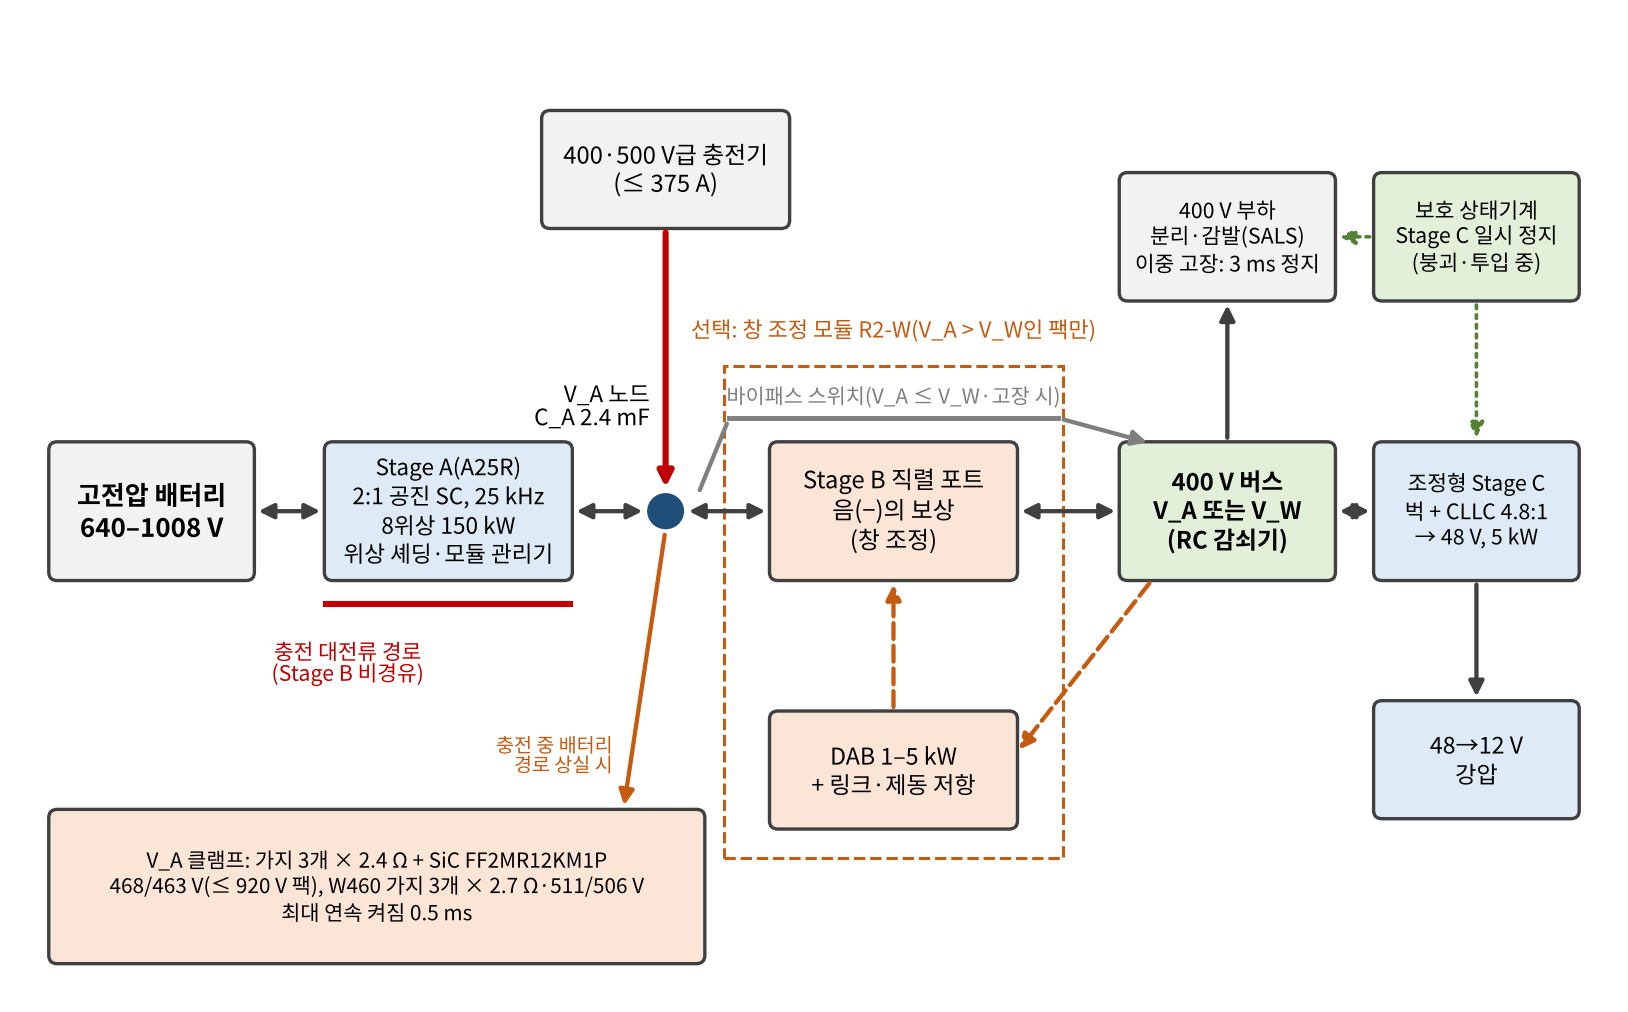
\includegraphics[width=16.0cm]{figs/fig1_r2_architecture.png}
\caption{PRISM-Hub 최종 구조(개선 구조 R2, Stage A A25R)의 전력 경로}\label{f:r2}
\srcnote{주: 상세보고서 Fig.~1. 640–1008 V는 사양 팩(640–920 V)에 고전압 팩(240s, 최대 1008 V)을 더한 표시 범위.}
\end{figure}

\section{Stage A: A25R 최종 설계}

Stage A는 공진전류의 영교차를 검출해 끄는 게이트로 영전류 스위칭을 유지한다. 25 kHz는 손실 모델을 바로잡은 결과로, 영전류 스위칭에서도 노드 용량의 전이당 손실은 E\textsubscript{oss}가 아니라 Q\textsubscript{oss}(V)·V다\cite{b32}. 이를 반영하면 150 kHz 원설계의 위상당 출력용량 손실은 175 W(이전 모델 14 W)였고, 영전류 게이트 조건에서 당시(E31)의 네 동시 기준(전압·전류 정격, 보조 손실, 충전 손실)을 통과한 24개 설계안(90안 중)은 모두 75 kHz 이하였다(150·100 kHz 0/30; 고주파 운전의 불가능이나 25 kHz의 유일성을 뜻하지 않음). 그 가운데 소자 수가 원설계 이하이면서 충전 손실이 가장 작은 25 kHz안(375 A 충전 0.52–0.64 kW)을 골랐다.

공진이 6배 느려지자 C\textsubscript{A} 400 µF(A25)에서는 느린 충전 과도 0/3이 불통과였고, C\textsubscript{A}를 6배(2.4 mF)로 키운 \textbf{A25R}이 최종 설계다. 그 대가로 충전 전 모든 모듈을 켜는 \textbf{사전 기동}과 \textbf{충전전류 증가 램프 600 µs 이상}을 요구한다. 경부하에서는 위상 셰딩(20 A 아래 600 µs에서 정지, 30 A 또는 순시 53 A에서 재가동)과 모듈 관리기(모듈당 70 A 추가, 60 A 감소)를 쓰고, 모듈 1개 고장은 그 모듈을 차단하고 남은 3개가 단기 인계한 뒤 충전 전류 지령을 3/4(281.25 A)로 재요청하도록 설계했다(재요청 뒤 충전기 응답은 모델 범위 밖). 영전류 스위칭(턴오프 전류 ≤ max(5 \% × 반주기 첨두, 1.0 A))과 위상 첨두 한도로 다시 판정한 결과, 요구 안 과도 6/6, 모듈 고장 16/16, 정상 운전점 공칭 33/36(정격 충전점 시작 과도 76.7 A)·공차 표본 36/36, 회로 TB27 4/4였다. 다만 요구 안 과도 6건 가운데 5건(느린 충전 3, 계단 2)은 수정안 선택에 쓴 사례이고, 요구 밖 조건(20 kW 순간 계단, 100 µs 램프, 사전 기동 없는 충전)은 불통과다.

\section{Stage B: 선택적 창 조정 모듈과 R1 제어기}

R2-W는 Eq.~(\ref{e:win})에 따라 운전한다.
\begin{equation}
V_\mathrm{bat}/2 \le V_\mathrm{W}-5~\mathrm{V}:\ \text{바이패스},\qquad
V_\mathrm{bat}/2 \ge V_\mathrm{W}+5~\mathrm{V}:\ V_\mathrm{bus}=V_\mathrm{W}
\label{e:win}
\end{equation}
바이패스 구간에서는 Stage B가 멈춰 고정 손실이 0이고, 창 조정 구간에서만 직렬 H-브리지의 음(−)의 보상으로 버스를 깎으며 DAB가 링크전력을 주고받는다. 제어기는 상세보고서에서 구현·검증한 \textbf{재설계 R1}이다. 모든 운전점에서 같은 고정 이득을 쓰는 표본화 상태궤환 제어기로, 제어주기 5 µs에 지령을 5 µs 뒤 적용하며 한 주기 예측으로 지연 여유를 4.1 µs(보상 없는 설계 1.4 µs)로 넓혔다.

\textbf{보호 상태기계}는 하드웨어 비교기·게이트 구동기 신호·링크전압 창으로 고장을 판단하며, H-브리지 고장은 바로 바이패스하면 수백 A가 흐르므로 그림~\ref{f:seq}의 순서로 강등한다. 전압비 불일치에서는 DAB를 1차 내부 위상천이(EPS)\cite{b2}로 바꾸고 지령표 첨두 상한은 정격점의 1.387배(전이 여유 포함)로 두었다. 회로 순시 수락 기준은 1.5배(R2-W460 68.7 A, R2-W410 90.0 A)다.

\begin{figure}[!tbp]
\centering
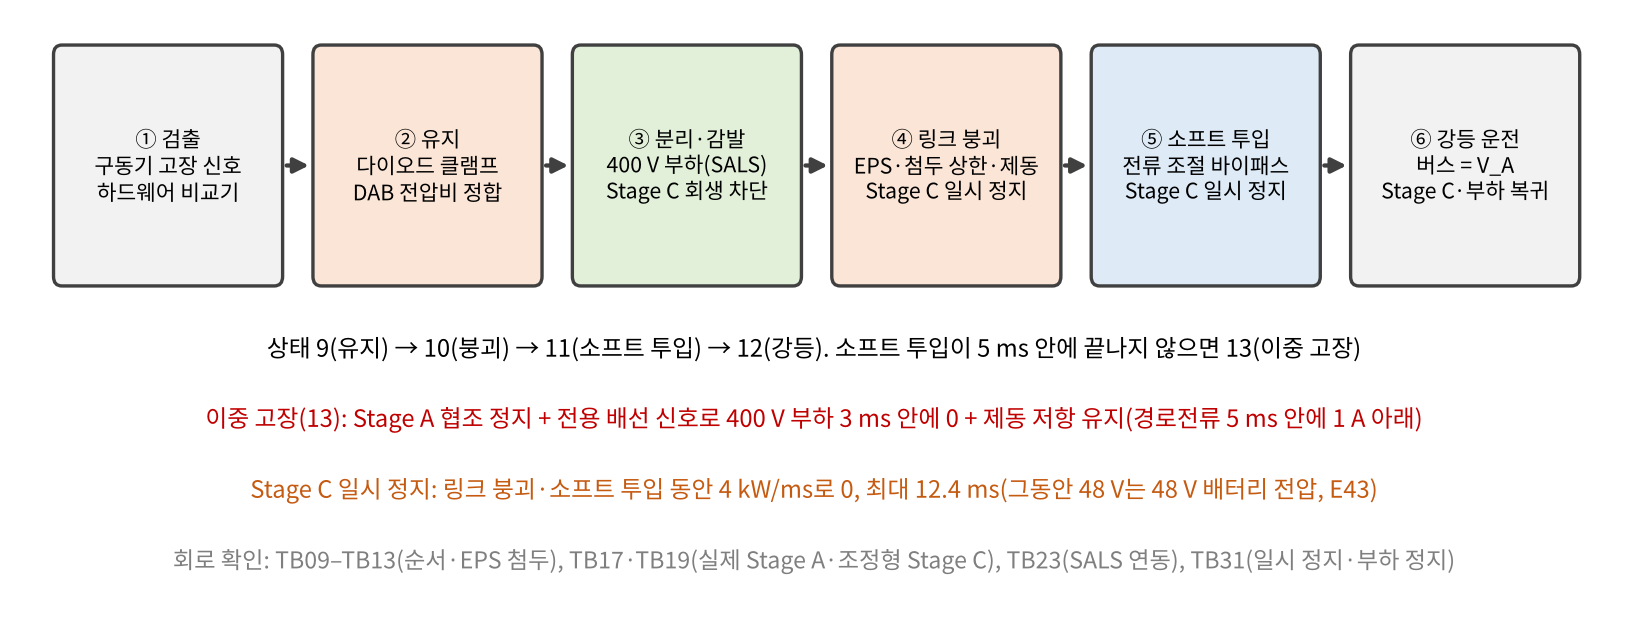
\includegraphics[width=16.0cm]{figs/fig2_fault_sequence.png}
\caption{창 조정 모듈 H-브리지 고장의 최종 강등 순서}\label{f:seq}
\srcnote{주: 상세보고서 Fig.~5. 최종 A25R과 한 회로로 결합해 확인하지는 않았다.}
\end{figure}

\section{Stage C와 부하 승인 계층(SALS)}

Stage C 입력은 270–504 V로 변해 고정이득 CLLC로는 48 V가 32.4–60.5 V로 무제한 운전 범위(36–52 V)\cite{b10}를 벗어나므로, 동기 벅과 공진점 고정 주파수 CLLC 직류변압기의 2단 구성을 택했다(공진점 CLLC는 양방향 이득이 1에 가깝다\cite{b17}). 전류·전압 PI와 앞먹임, 출력전류 제한(과도 130 A, 2 ms 뒤 105 A)을 쓴다.

SALS는 상위 부하 승인 계층으로, 향후 160 ms 최악 합이 예산(23.75 kW) 이하일 때만 부하를 승인한다. 보호 상태기계는 강등 뒤 버스가 부품 상한을 넘는 팩에서는 400 V 부하를 바로 분리하고, 상한 이내에서는 SALS로 감발을 명령해 감발이 확인되면 부하를 복원하며 30 ms 안에 확인되지 않으면 접촉기로 분리한다. 또 H-브리지 고장 강등의 링크 붕괴·소프트 투입 동안 Stage C를 4 kW/ms로 줄여 최대 12.4 ms 멈춘다(\textbf{보호 일시 정지}). 이중 고장에서는 Stage A를 멈추고 400 V 부하를 3 ms 안에 0으로 줄인다.

\chapter{검증 체계}\label{s:method}

검증은 해석, 평균모델, 스위칭 모델, MATLAB/Simulink Simscape 소자 수준 회로(TB01–TB33, 기생성분·열 제외)로 했다(근거 E1–E47). 부하 계단은 Tier-1(대표 변화)과 Tier-2(1→25 kW)로 나누고, 전류 기준은 평균모델 90·93.75 A, 스위칭·회로 모델 98·100 A(순시값)다. 최종 A25R은 정적 등가 재계산과 회로 TB27·TB28·TB33으로 확인했고, Stage B 보호 회로는 V\textsubscript{A}를 이상 전원으로 두었으며, Stage A와 조정형 Stage C를 한 회로에 넣은 TB16–TB19(Stage B까지 넣은 것은 TB17·TB19)는 150 kHz Stage A 1모듈이다. \textbf{최종 A25R·Stage B·Stage C와 최종 보호 순서 전체를 결합한 단일 회로는 없다.}

\chapter{설계 성능과 검증 결과}

\section{충전 경로와 전력 정격 분리(H1)}

초기 전 범위 Stage B(DAB 8 kW)의 주행 중 링크전력은 25 kW 정상상태 전력수지(E3, 640 V)에서 최대 6.44 kW, 사양 팩 640–920 V 과도 시험 516건에서 7.16 kW, 640 V 복합 공차(±10 \%) 256건에서 7.12 kW였다. 같은 Stage B를 A25R 정적 등가로 다시 계산한 충전 중 링크전력은 사양 640–920 V에서 정적 6.29 kW, 과도 7.04 kW였다(632 V 경계 진단 포함 시 6.69·7.49 kW). 이전 150 kHz Stage A 회로(TB07)에서도 충전전류 375 A는 V\textsubscript{A} 노드에서 Stage A로 들어가고 Stage B 경로전류는 보조부하분인 13–79 A였다. \textbf{판정: H1 충족}(Stage B가 있는 구조).

800 V·375 A 충전 경로 손실은 Stage A가 0.59 kW로 같은 손실 규칙의 전용 승압기(50 kHz) 1.77 kW보다 작았다. 전용 승압기 16–50 kHz 기준으로는 0.32–0.51배, 상저항 10 mΩ의 모터 승압 기준점에 대해서는 약 절반이고, 상저항 5 mΩ 하한과는 0.92–1.02배로 같은 수준이다. 이 이점은 \textbf{충전 경로에 한정}되며 전체 손실 우위를 뜻하지 않는다(\ref{s:h5}절).

\section{제어 안정성과 강건성(H2)}

단일 공차 격자에서 Tier-1은 460/460, Tier-2는 78/78(추가 지연 제외; +3 µs 정보 시험 13/14)이었다. 640 V에서 7개 파라미터를 각각 ±10 \% 끝값으로 바꾼 128개 조합의 Tier-2 결과는 Table~\ref{t:h2}와 같다.

\Needspace{7\baselineskip}
{\footnotesize
\begin{longtable}{L{\dimexpr 0.36\linewidth-2\tabcolsep\relax}L{\dimexpr 0.18\linewidth-2\tabcolsep\relax}L{\dimexpr 0.12\linewidth-2\tabcolsep\relax}L{\dimexpr 0.34\linewidth-2\tabcolsep\relax}}
\caption{640 V 복합 공차 Tier-2(128개 조합)의 모델별 결과}\label{t:h2}\\
\toprule
\tabhead \textbf{모델·시험} & \textbf{전류 기준} & \textbf{통과} & \textbf{최대값·비고} \\
\midrule
\endfirsthead
\toprule
\tabhead \textbf{모델·시험} & \textbf{전류 기준} & \textbf{통과} & \textbf{최대값·비고} \\
\midrule
\endhead
\bottomrule
\endlastfoot
평균모델(정식 판정) & 93.75 A & \textbf{102/128} & 최대 95.82 A \\
스위칭 모델 & 순시 100 A & 128/128 & 최대 97.32 A \\
스위칭 모델 + 추가 지연 +3 µs(별도 시험) & 순시 100 A & 114/128 & 실패 100.05–101.21 A. 128/128과 합산하지 않음 \\
\end{longtable}
}

평균모델과 스위칭 모델은 전류 기준이 달라 같은 척도로 비교할 수 없고, 시험 전에 정한 평균모델 기준에서는 26건이 불통과였다. +3 µs 시험은 같은 조합에 추가 지연을 준 별도 시험이다. 별도로 창 조정 모듈 R2-W460·R2-W410은 이전 150 kHz Stage A 등가(전압원 + 경로 저항 13.2 mΩ)의 평균모델에서 공차·지연 +3.0 µs를 포함한 Tier-1·Tier-2 합계 R2-W460 456/456, R2-W410 264/264를 통과했으나, A25R과 결합해 재시험한 결과는 아니다. \textbf{판정: H2 부분 충족}(Stage B 모델 범위).

\section{충전 중 보조버스 운전(H3)}

충전(375 A 제한)과 보조부하 25 kW의 동시 운전, 충전기 접속·해제를 최종 설계로 다시 계산한 평균모델(정적 등가; 모든 판정량에서 보수적이라는 증명은 없음)로 확인했다(Table~\ref{t:h3}). A25R 회로 확인은 시험별로 범위가 다르다: 보조 15 kW 결합 회로(TB28 D28)의 800 V 충전 시작·종료, 보조 25 kW 결합 회로(이전 단일 1 Ω 클램프, TB28 A28·B28·C28)의 경로 상실 뒤 충전전류 0에서 1 ms·모듈 고장 뒤 2 ms 관찰, Stage A 회로 TB27 4/4, 별도 Stage A 모델의 640 V·15·25 kW 600 µs 램프.

\Needspace{7\baselineskip}
{\footnotesize
\begin{longtable}{L{\dimexpr 0.22\linewidth-2\tabcolsep\relax}L{\dimexpr 0.44\linewidth-2\tabcolsep\relax}L{\dimexpr 0.34\linewidth-2\tabcolsep\relax}}
\caption{충전 중 보조버스 시험(A25R 정적 등가, 평균모델)}\label{t:h3}\\
\toprule
\tabhead \textbf{시험} & \textbf{조건} & \textbf{결과} \\
\midrule
\endfirsthead
\toprule
\tabhead \textbf{시험} & \textbf{조건} & \textbf{결과} \\
\midrule
\endhead
\bottomrule
\endlastfoot
동시 운전 Tier-1 & 460건(632 V 경계 진단 20건, 공차·지연 +3.0 µs 포함), 부하 스텝 10가지 & 460/460(사양 640–920 V만 440/440) \\
동시 운전 Tier-2 & 78건(632 V 2건 포함, +3 µs 정보 시험 제외), 스텝 1↔25 kW & 78/78(사양 76/76), 최대 92.7 A \\
모드 전환 & 충전기 접속·해제 등 240건 & 240/240, 경로 ≤ 86.3 A \\
전체 운전 순서 & 30건 & 30/30, 버스 397.81–401.44 V \\
\end{longtable}
}

\textbf{판정: H3 충족(조건 있음).} 조건은 충전 전 사전 기동과 충전전류 증가 램프 600 µs 이상이며(램프 조건은 보조부하 15·25 kW에서 확인), 판정은 보조부하 25 kW에서 했다. 같은 기동·램프에서 640 V·보조부하 0·1 kW는 위상 첨두 78.63·78.74 A로 한도 74.53 A를 넘어 경부하 기동의 한계가 남았다. 또 충전기 명령은 Eq.~(\ref{e:ich})의 입력 한계이므로 모든 배터리 전압에서 150 kW가 전달된다는 뜻이 아니다.
\begin{equation}
I_\mathrm{chg}=\min\!\left[375~\mathrm{A},\ \frac{150~\mathrm{kW}}{V_\mathrm{bat}/2}\right]
\label{e:ich}
\end{equation}

\section{Stage C 48 V 조정 성능}

평균모델(입력 270·330·400·460·504 V)에서 정상 조정 오차는 0.000 \%(기준 ≤ 0.1 \%), 48 V 설정의 계약 부하 변화 4 kW/ms 최대 편차는 \textbf{0.49 \%}, 버스 계단 ±50 V/10 µs는 0.59 \%, 방향 전환 −3 → +3 → −3 kW는 0.22 \%로 과도 세 항목 모두 ±2 \% 안이었다. 이와 별도로 48 V 배터리를 뺀 극한 계단(0.1↔5 kW, −3↔+5 kW)에서는 ±2 \%를 벗어나지만 40.64–50.91 V로 36–52 V 안에 머물렀다(제어 시험 8종 모두 통과). 그 가운데 −3 → +5 kW 계단의 응답이 그림~\ref{f:e22}이다.

\begin{figure}[!htbp]
\centering
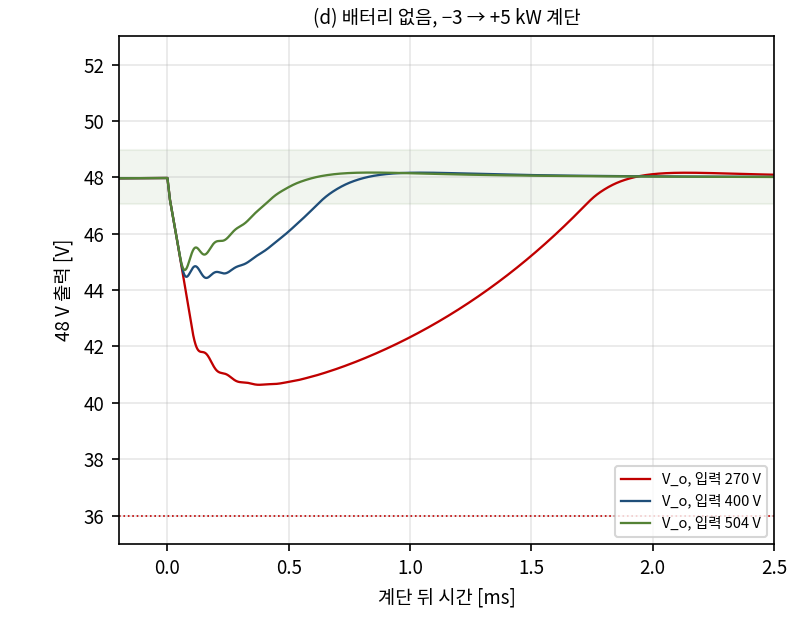
\includegraphics[width=11.0cm]{figs/fig4_stagec_step_d.png}
\caption{Stage C 48 V 출력의 극한 부하 계단 응답(배터리 없음, −3 → +5 kW, 평균모델)}\label{f:e22}
\srcnote{주: 상세보고서 Fig.~8(E22)의 패널 (d)를 잘라 그대로 확대했다(데이터·파형 변경 없음). 입력 270·400·504 V, 음영은 48 V ±2 \%, 붉은 점선은 36 V. 48 V 배터리를 뺀 극한 계단 시험으로, 계약 부하 변화(4 kW/ms)의 최대 편차 0.49 \%와는 시험 조건이 다르다.}
\end{figure}


소자 수준 회로에서는 레그 출력용량을 반영해 자화 인덕턴스(33 µH)와 데드타임(1차 100 ns·2차 40 ns)을 정하고 경부하에서 두 브리지를 함께 구동했다(첫 회로 TB14 1차는 0/5). 최종 회로 \textbf{TB15는 5/5}로, 각 브리지 대표 레그의 지정 정상 시간창에서 켜짐 직전 소자 전압이 \textbf{0.22 V 이하}였고 회생 전환 사례의 48 V는 47.79–48.07 V였다. 5 kW 최악 손실은 \textbf{170.3 W(효율 약 96.7 \%)}로 모델 추정값이며 측정 효율이 아니다.

따라서 Stage C는 R2의 넓은 입력 범위에서 48 V 조정을 맡을 수 있다. 다만 CV 설정 범위 36–52 V 전체는 보장하지 않으며(입력 270 V·출력 52 V·−650 W 단측 송신 정상점, 두 브리지 출력용량 +20 \%에서 필요 듀티 0.980 > 0.97), 일시 정지 중 48 V는 배터리 등가 계산(41.6–45.7 V, ±2 \% 조정은 유지되지 않음)일 뿐 회로에 배터리를 구현한 결과가 아니다.

\section{보호·고장 강등과 부하 승인(H4)}

\textbf{H-브리지 개방 고장.} 평균모델(E17)에서 즉시 바이패스는 R2-W460·R2-W410 각각 0/4(최대 766·869 A), 초기 추천 순서(클램프 유지 + 제동)는 각각 4/4(경로 ≤ 90.0·90.3 A)였고, 그림~\ref{f:seq}의 최종 순서는 여기에 EPS·첨두 상한·일시 감발·Stage C 일시 정지를 더한 것이다. V\textsubscript{A}를 이상 전원으로 둔 Stage B 회로(TB09)의 첫 실행에서는 링크가 내려가지 않아 소프트 투입 중 경로전류가 177 A까지 올랐다. 붕괴 정체 감지·전류 조절 투입을 넣어 회로 4/4를 얻었다(TB09). 이어 EPS 변조를 넣고 지령표 상한을 1.387배로 낮춰 회로 첨두 1.5배 기준을 통과했고(TB13 2/2; TB11 0/2·TB12 1/2를 거침), EPS는 링크 5 V·11 A 운전점의 첨두를 189 A에서 20 A로 줄였다.

\textbf{SALS 연동·이중 고장·클램프.} 메시지 지연·손실 74개 조합(74/74)과 이중 고장 3 ms 정지(4/4)에서 강등이 성립했다. Stage C 일시 정지를 넣은 뒤 소프트 투입 최악 에너지는 0.036 J, 바이패스 GaN 접합온도는 109.6 °C(전형값 보수 규칙 L, 이전 규칙 108.0 °C)였다. 충전 중 배터리 경로를 잃으면 V\textsubscript{A}가 충전기 전류로 올라가므로(920 V 충전에서 클램프 없이 0.06–0.09 ms에 470 V 도달) 클램프가 필요하다. 최종 클램프 회로(TB33)는 무부하 경로 상실 두 사례를 통과했지만(회로 V\textsubscript{A} 468.14 V·버스 ≤ 469.03 V, 평균모델과 0.2 A·0.3 J 안), \textbf{오동작 사례 C33은 불통과}였다. 회로는 9 µs 만에 클램프를 껐지만 평균모델은 0.5 ms 동안 켜져 있어(3.3 J 대 177.6 J) 대조를 통과하지 못했다. 정격 보조부하를 건 경로 상실은 이전 단일 1 Ω 클램프 회로(TB28)에서만 확인했다.

\textbf{부하 승인(H4).} 200개 × 20 s 축약 시나리오에서 예산 초과는 0 ms였다. 압축기 승인 지연은 메시지 무손실 100개 시나리오(235건)에서 최대 17 ms, 메시지별 독립 손실 0–20 \% 100개 시나리오(253건)에서 99백분위 25.44 ms(최대 32 ms)로 기준(25·50 ms) 안이었고, 미공급률(지연 가능 히터 두 종의 요청 에너지 기준)은 6.96 \%로 정적 예약 방식(35.21 \%)보다 작았다. \textbf{판정: H4 충족}(축약 모델).

\section{구조 비교와 H5}\label{s:h5}

같은 서비스(충전 375 A, 보조부하 최대 23 kW, 48 V 평균 1.5 kW), 같은 손실 규칙과 주행 대표 프로파일(760–900 V)로 다섯 구조를 비교했다. 보조부하는 대부분 경부하에서 운전하므로 고정 손실이 평균 손실을 좌우한다\cite{b11}(Table~\ref{t:h5}).

\Needspace{8\baselineskip}
{\footnotesize
\begin{longtable}{L{\dimexpr 0.40\linewidth-2\tabcolsep\relax}L{\dimexpr 0.17\linewidth-2\tabcolsep\relax}L{\dimexpr 0.15\linewidth-2\tabcolsep\relax}L{\dimexpr 0.12\linewidth-2\tabcolsep\relax}L{\dimexpr 0.16\linewidth-2\tabcolsep\relax}}
\caption{기준 구조의 손실·정격 비교(사양 팩, 주행 대표 프로파일)}\label{t:h5}\\
\toprule
\tabhead \textbf{구조} & \textbf{보조 경로 평균 손실} & \textbf{375 A 충전 손실} & \textbf{스위치 위치} & \textbf{스위치 VA} \\
\midrule
\endfirsthead
\toprule
\tabhead \textbf{구조} & \textbf{보조 경로 평균 손실} & \textbf{375 A 충전 손실} & \textbf{스위치 위치} & \textbf{스위치 VA} \\
\midrule
\endhead
\bottomrule
\endlastfoot
① 전전력 승압기 + 800→400 V 강압기 & 112.4 W & 1.77 kW & 24 & 818 kVA \\
② Stage A + 전전력 조정기 & 134.6 W & 0.59 kW & 44 & 1,096 kVA \\
③ 초기 구조(전 범위 Stage B) & 144.5 W & 0.59 kW & 52 & 1,099 kVA \\
③′ 창 조정(버스 ≤ 410 V) & 130.4 W & 0.59 kW & 56 & 1,131 kVA \\
\textbf{④ 비조정(R2 기본형)} & \textbf{101.5 W} & \textbf{0.59 kW} & \textbf{42} & \textbf{1,009 kVA} \\
\end{longtable}
}
\srcnote{주: 설계 단계 손실 규칙의 상대 비교(측정 아님). 충전 손실은 800 V, ①은 50 kHz 전용 승압기. ①의 보조 강압기는 셰딩 없이 계산했다.}

\textbf{판정: H5 기각.} 초기 구조 ③은 비조정 구조 ④보다 보조 경로 손실(144.5 대 101.5 W), 스위치 VA, 스위치 위치가 모두 컸다. 원인은 Stage B의 경부하 고정 손실이다. 직렬전압이 0 근처여도 H-브리지는 경로전류 전체를 흘리며 스위칭하고 DAB는 영전압 스위칭을 잃어 약 65 W(DAB 무부하 45.8 W, H-브리지 약 19.5 W)를 쓰며, 이는 48 V 조정을 Stage C로 옮긴 대가(약 22 W)보다 크다. 또 직렬 ±90 V로는 V\textsubscript{A} 약 310–490 V만 400 V로 맞출 수 있어 셀 180–240s 가운데 216·224s 팩에서만 전 범위 조정이 성립했다. 그래서 Stage B를 필요한 팩에만 두는 선택 모듈로 바꿨다.

% 손실 비교 그림을 4.6절 끝에 고정 배치한다.
{\setlength{\intextsep}{6pt plus 2pt minus 2pt}
\begin{figure}[H]
\centering
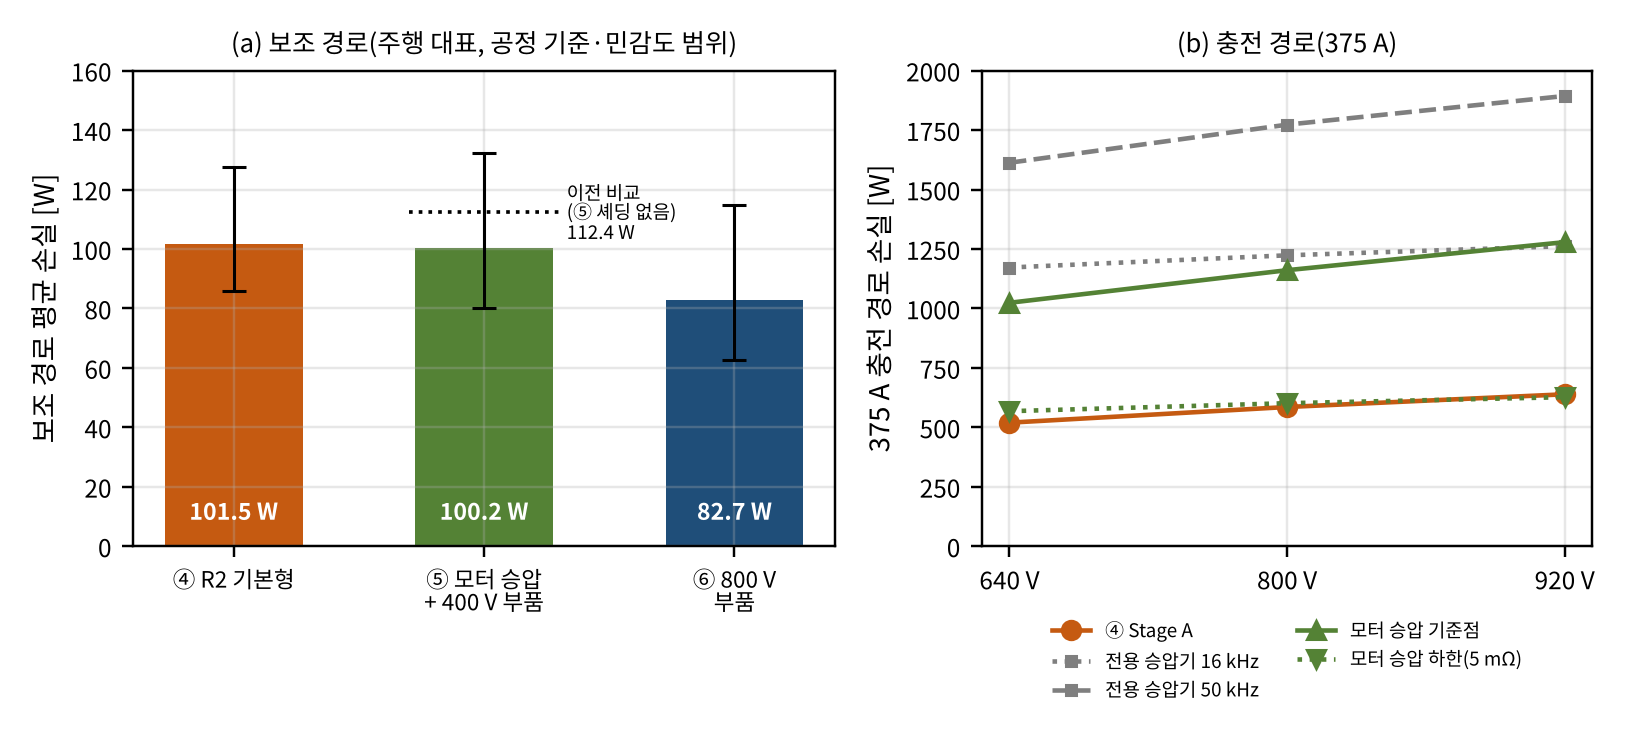
\includegraphics[width=16.0cm]{figs/fig3_loss_comparison.png}
\caption{산업 방식 대비 보조 경로와 충전 경로 손실(최종 설계, 공정 기준)}\label{f:loss}
\srcnote{주: 상세보고서 Fig.~16. (a) 오차막대는 민감도 범위, (b) 375 A 충전 경로(전용 승압기 16·50 kHz, 모터 승압 기준점·하한 5 mΩ). ⑤·⑥은 모터 승압 + 400 V급·800 V급 보조부품. ⑤는 셰딩 적용 100.2 W, 점선은 셰딩 없는 112.4 W.}
\end{figure}
}

그림~\ref{f:loss}는 상용 적용 사례가 있는 모터·인버터 승압\cite{b24,b25} 등 산업 방식과의 \textbf{공정 기준} 비교다. ①과 모터 승압 방식 ⑤는 같은 보조 강압기를 쓰며, Table~\ref{t:h5}에서는 경부하에도 2위상을 유지해 112.4 W였다. ④는 Stage A 위상 셰딩을 쓴다. 주행 시간의 60 \%가 0.5–2.5 kW여서 경부하 기법의 유무가 평균 손실을 좌우한다. 공정 기준에서는 ①·⑤의 강압기도 운전점마다 손실이 작은 1·2위상을 선택해 100.2 W가 된다. 두 값은 셰딩 가정만 다르고 운전 프로파일과 손실 규칙은 같다. 공정 기준에서 R2 기본형은 ⑤와 같은 수준(101.5 대 100.2 W, 민감도에 따라 부호가 바뀜)이고 800 V급 보조부품 설계 ⑥보다 4–33 W 크며, 창 조정 모듈이 최소였던 세 칸(B\textsubscript{420} 200s, B\textsubscript{470} 224·240s)도 공정 기준에서는 다른 성립 구조와 같은 수준이어서 손실 이점이 없다. 따라서 \textbf{R2의 의미는 무조건적인 효율 우위가 아니라}, 충전 경로 손실의 이점과 함께 필요한 전압 조건에서만 조정 기능을 두어 구조를 성립시키고 보호·고장 강등을 구현하는 데 있다.



\chapter{결론과 한계}

최종 판정은 Table~\ref{t:status}와 같다(해당 모델·조건 안에서만 유효).

\Needspace{8\baselineskip}
{\footnotesize
\begin{longtable}{L{\dimexpr 0.23\linewidth-2\tabcolsep\relax}L{\dimexpr 0.19\linewidth-2\tabcolsep\relax}L{\dimexpr 0.58\linewidth-2\tabcolsep\relax}}
\caption{가설과 연구 질문 Q3의 최종 판정}\label{t:status}\\
\toprule
\tabhead \textbf{가설} & \textbf{판정} & \textbf{핵심 근거} \\
\midrule
\endfirsthead
\toprule
\tabhead \textbf{가설} & \textbf{판정} & \textbf{핵심 근거} \\
\midrule
\endhead
\bottomrule
\endlastfoot
H1 정격 분리 & 충족(Stage B가 있는 구조) & 전 범위 Stage B 링크 ≤ 7.16 kW(충전 중 ≤ 7.04 kW), 충전전류 Stage B 비경유 \\
H2 강건 제어 & 부분 충족(Stage B 모델 범위) & Tier-2 평균모델 102/128, 스위칭 128/128, +3 µs 별도 114/128 \\
H3 충전 중 보조버스 & 충족(조건: 사전 기동·램프) & 사전 기동·램프 ≥ 600 µs(보조 15·25 kW에서 확인, 판정 25 kW), 640 V·0–1 kW 기동은 78.63–78.74 A > 74.53 A \\
H4 부하 승인 & 충족(축약 모델) & 예산 초과 0 ms, 미공급 6.96 \%(정적 35.21 \%) \\
H5 기준 구조 대비 이점 & 기각 & 보조 손실 ③ 144.5 대 ④ 101.5 W \\
Q3 산업 방식 대비 & 제한적 & 충전 경로 손실만 이점, 보조 손실은 ⑤와 같은 수준·⑥보다 4–33 W 큼 \\
\end{longtable}
}

한계는 (1) 하드웨어 실측 없음(손실·효율은 모델 추정), (2) 최종 설계 전체의 결합 회로 없음, (3) H2 복합 공차·H3 경부하 기동·Stage C CV 전 범위, (4) TB33 C33 불통과와 일시 정지 중 48 V 배터리 연동, (5) 클램프 문턱 구현 요구와 실제 켬·끔 지연(0.5 µs에서 사양 팩 폭 3.5 V가 151.26 °C로 한도 초과)·조건부 부품, (6) 새 인터페이스 요구(Stage C 일시 정지, 400 V 부하 3 ms 정지)의 실제 응답, (7) 정적 등가의 보수성 미증명과 A25R 회로와 결합해 다시 확인하지 않은 Stage B 보호·강등 시험이며, 하드웨어 실증이 다음 과제다.

결론적으로 Q1은 긍정(기존 전 범위 Stage B의 링크전력 8 kW 이내, 검증한 정상·계약 과도 조건에서 48 V 편차 ±2 \% 이내; 보호 일시 정지 중에는 배터리 등가 전압을 따름), Q2는 부분 긍정, Q3는 초기 구조 부정·R2 제한적이다. 전 범위 정밀 조정이 경부하 고정 손실로 이점을 잃는다는 부정적 결과가 필요한 조건에서만 조정하는 R2를 낳았고, 영전류 스위칭 공진 단에서도 Q\textsubscript{oss}·V 손실이 설계를 좌우할 수 있어 25 kHz 설계는 V\textsubscript{A} 노드 커패시터와 충전 램프 요구를 함께 바꿔야 성립했다. R2는 400 V급 보조부품을 그대로 쓰는 차량에서 충전 손실을 줄이는 선택지이며, V\textsubscript{A}가 부품 상한을 넘는 팩에서는 창 조정 모듈이 성립 수단이 된다.
